	%After first compiling run following commands in command prompt and compile again:
	%bibtex Proposal - where Proposal is the name of your main file
	%makeglossaries Proposal - where Proposal is the name of your main file
	
	%\documentclass[twoside, openright, a4paper,12pt]{report} % Two side 
	\documentclass[oneside,a4paper,12pt]{book} 
	\usepackage{pdfpages}
	\usepackage{JMTemplate}
	\usepackage{tikz}
	\usepackage{pgfplots}
	\usetikzlibrary{automata,positioning}
	\usepackage{amsthm}
	\usepackage{amssymb}
	\usepackage[]{amsmath}
	\usepackage{dsfont}
	\usepackage{pgfplots}
	\usepackage{color}
	\usepackage{multirow}
	\definecolor{darkgreen}{RGB}{47,109,79}
	\definecolor{darkblue}{RGB}{57,79,99}
	\definecolor{rosso}{RGB}{220,57,18}
	\definecolor{giallo}{RGB}{255,153,0}
	\definecolor{blu}{RGB}{102,140,217}
	\definecolor{verde}{RGB}{16,150,24}
	\definecolor{viola}{RGB}{153,0,153}
	\definecolor{awesome}{rgb}{1.0, 0.13, 0.32}
	\definecolor{ref}{rgb}{0.65,0.65,0.65} %{0.4,0.8,0.85}
	\definecolor{highlightrow}{rgb}{0.9,0.9,0.9}
	
	\newcommand{\norm}[1]{\left\lVert#1\right\rVert}
	
	% Information for pdf making 
	%=======================================================
	\newcommand{\fatype}{پایان‌نامه}
\newcommand{\fatitle}{تولید دنباله با استفاده از شبکه‌های مقابله‌ای}
\newcommand{\faAuthor}{احسان منتها‌ئی}
\newcommand{\fasupervisor}{دکتر مهدیه سلیمانی}
\newcommand{\fadate}{زمستان ۱۳۹۷}
\newcommand{\famajor}{گرایش هوش مصنوعی}
\newcommand{\falevel}{کارشناسی ارشد}
\newcommand{\fadepart}{دانشکده مهندسی کامپیوتر}

\newcommand{\entype}{Thesis}
\newcommand{\entitle}{Adversarial Networks for Sequence Generation}
\newcommand{\enAuthor}{Ehsan Montahaei}
\newcommand{\ensupervisor}{Dr. M. Soleymani}
\newcommand{\engdate}{Winter 2018}
\newcommand{\enmajor}{Artificial Intelligence}
\newcommand{\enlevel}{M.Sc.}
\newcommand{\enDep}{Department of Computer Engineering}

\newcommand{\momtaheninFirst}{دکتر حسین صامتی}
\newcommand{\momtahenouFirst}{دکتر عمادالدین فاطمی‌زاده}



	\hypersetup{
		pdftitle={\entitle} 
		,pdfauthor ={\enAuthor}
		,pdfsubject={\enlevel{} \entype{} (\enmajor), \enDep, Sharif University of Technology, Tehran, Iran}
	}
	
	\glsdisablehyper % disable hyperlinks

\newglossarystyle{persian-to-english}{%
%	\glossarystyle{listdotted}% the base style
	% put the glossary in a two column page and description (as in listdotted style) environment:
	\renewenvironment{theglossary}%
		{\begin{multicols}{2}\begingroup \flushleft }%
		{\endgroup \end{multicols}}%
%	\renewenvironment{theglossary}{}{}%
	% have nothing after \begin{theglossary}:
	\renewcommand*{\glossaryheader}{}%
	% have nothing between glossary groups:
	\renewcommand*{\glsgroupheading}[1]{}%
	\renewcommand*{\glsgroupskip}{}%
	% set how each entry should appear: \glossaryentryfield{label}{formatted name}{description}{symbol}{number list}
	\renewcommand*{\glossaryentryfield}[5]{%
		\glstarget{##1}{##2}% persian term
		\dotfill%dots
		\space \lr{##3} \\%
%		\dotfill%
%		\space {##5} \\%translation term
	}%
	% set how sub-entries appear:
	\renewcommand*{\glossarysubentryfield}[6]{%
		\glossaryentryfield{##2}{##3}{##4}{##5}{##6}%
	}%
}
% ========= Glossary styles (put in files) =========
\newglossarystyle{english-to-persian}{%
%	\glossarystyle{listdotted}% the base style
	% put the glossary in a two column page and description (as in listdotted style) environment:
	\renewenvironment{theglossary}%
		{\begin{multicols}{2}\begingroup \flushright }%
		{\endgroup \end{multicols}}%
%	\renewenvironment{theglossary}{\Latin{}}{\Persian{}}%
	% have nothing after \begin{theglossary}:
	\renewcommand*{\glossaryheader}{}%
	% have nothing between glossary groups:
	\renewcommand*{\glsgroupheading}[1]{}%
	\renewcommand*{\glsgroupskip}{}%
	% set how each entry should appear:
	\renewcommand*{\glossaryentryfield}[5]{%
		\glstarget{##1}{##2}% persian term
		\dotfill%dots
		\space \rl{##3} \\%translation term
	}%
	% set how sub-entries appear:
	\renewcommand*{\glossarysubentryfield}[6]{%
		\glossaryentryfield{##2}{##3}{##4}{##5}{##6}%
	}%
}

% ========= GLOSSARIES =========
\newglossary{p2e-terms}{fa.gls}{fa.glo}{واژه‌نامه فارسی به انگلیسی} % persian to english
\newglossary{e2p-terms}{en.gls}{en.glo}{English to Persian Glossary} % english to persian

\newcommand{\newtrans}[3][]{% params: persian, english translations, first optional is a key
\newtranspl[#1]{#2}{#3}{#2‌ها}%
}

\newcommand{\newtranspl}[4][]{% params: persian, english, plural form of persian, first optional is a key
\ifthenelse{\isempty{#1}}{\def\key{#2}}{\def\key{#1}}%
\newglossaryentry{en:\key}{type={e2p-terms}, name={#3}, description={#2}}% english glossary
%	\newglossaryentry{fa:\key}{type={p2e-terms}, name={#2}, description={#3}}% persian glossary
\newglossaryentry{fa:\key}{type={p2e-terms}, name={#2}, plural={#4}, description={#3}}% persian glossary
}
% ========= END OF GLOSSARIES =========

% Show a translation and footnote it.
% Params (the same as \glsdisplayfirst):{text}{description}{symbol}{insert}
% insert can possibly be filled with some notes on the translation.
\newcommand{\showTransFirst}[4]{%  translation for the first time
\ifthenelse{\isempty{#4}}%
{\textit{#1}\LTRfootnote{ #2}}% if #4 is empty (no notes) 
%%%{\textit{#1}\LTRfootnote{{#2} #4}}% if #4 is not empty
{\textiranic{#1}\LTRfootnote{{#2} #4}}% if #4 is not empty
%{\textit{#1}\footnote{ \lr{#2}؛  #4}}% if #4 is not empty
}

\newcommand{\showTrans}[4]{% translation for next times
\ifthenelse{\isempty{#4}}%
{{#1}}% if #4 is empty (no notes) 
{\textit{#1}\footnote{#4}}% if #4 is not empty
}

\defglsdisplayfirst[p2e-terms]{\showTransFirst{#1}{#2}{#3}{#4}}% protect fragile commands
\defglsdisplay[p2e-terms]{\showTrans{#1}{#2}{#3}{#4}}

% Symbol may temporarily used to keep some notes on the translation.
% It must be replaced with a user1 key which now raises error, texlive must be upgraded.
\newcommand{\term}[2][]{%
\glsadd{en:#2}%
\ifthenelse{\isempty{#1}}{\gls{fa:#2}}{\gls{fa:#2}[#1]}%
}
\newcommand{\termpl}[2][]{%
\glsadd{en:#2}%
\ifthenelse{\isempty{#1}}{\glspl{fa:#2}}{\glspl{fa:#2}[#1]}%
}
%=========== Print Glossaries ===============
% see: http://www.parsilatex.com/forum/SMF/index.php?topic=345.0
%\glossarystyle{persian-to-english}
%\def\glossaryname{واژه‌نامه فارسی به انگلیسی}
%\printglossaries

\newcommand{\printpersianglossary}[1][واژه‌نامه فارسی به انگلیسی]{{%
	\phantomsection % hyperref: enable hyperlinking from the table of contents to this point
	\addcontentsline{toc}{chapter}{#1} % add a line in the Table of Contents (first option, toc), it will be like the ones 
	\renewcommand{\glossarymark}[1]{\markboth{##1}}% correct handling of page header
	\printglossary[type={p2e-terms},style={persian-to-english},title={#1}]%
}}


\newcommand{\printenglishglossary}[1][واژه‌نامه انگلیسی به فارسی]{{%
	\phantomsection % hyperref: enable hyperlinking from the table of contents to this point
	\addcontentsline{toc}{chapter}{#1} % add a line in the Table of Contents (first option, toc), it will be like the ones 
	\renewcommand{\glossarymark}[1]{\markboth{##1}}% correct handling of page header
	\begin{latin}%
	\printglossary[type={e2p-terms},style={english-to-persian},title={\rl{#1}}]%
	\end{latin}%
}}

% Reset the first-use flag of the transaltion glossareis
\newcommand{\resettranslations}{\glsresetall[e2p-terms,p2e-terms]} %This file wasR prepared by Sadegh Dorri
	\makeglossaries
	% Begin of document
	%=======================================================
	\begin{document}
		\pagestyle{fancy}
\fancyhead{}
%\fancyfoot{\hline\scriptsize\lr{\copyright} کلیه حقوق این سند محفوظ بوده و متعلق به آزمایشگاه رسانه دیجیتال دانشگاه صنعتی شریف  می‌باشد.}
\lhead{تولید دنباله با استفاده از شبکه‌های مقابله‌ای  - \thepage}
\rhead{}
\lfoot{}
\rfoot{}
		\dominitoc %initialization of minitoc
		\bstctlcite{Proposal:BSTcontrol} % activate IEEEtran_biboptions.bib options
		% Front matter
		%=======================================================
		\begin{center}
\thispagestyle{empty}

\includegraphics{logo}

\begin{large}
دانشگاه صنعتی شریف \\ \fadepart{}
\vskip 0.8cm
\fatype{} \falevel{} \\ \famajor{}

\end{large}
\vskip 2cm
{\large{عنوان}} 
\vskip 0.5cm
{\titlefont{\textbf{\fatitle}}}
\vskip 2 cm
\large{نگارش} \\ \Large{\faAuthor}
\vskip 0.75cm
\large{استاد راهنما} \\ \Large{\fasupervisor}
\vskip 2cm
\large{\fadate}
\end{center}


		\cleardoublepage % terminates the current paragraph and page, the same way as a report document.
		\thispagestyle{empty}
\begin{center}
\Large{دانشگاه صنعتی شریف} \\
\Large{\fadepart}
\vskip 1cm
\large{\fatype{} \falevel}
\vskip 2cm
\textbf{\Large{\fatitle}}
\vskip 2cm
نگارش: \faAuthor
\end{center}
\vskip 4cm
\begin{tabular}{p{3cm}p{6.5cm}p{5cm}}
استاد راهنما:&
\fasupervisor  &
امضاء: \\[2cm]
استاد ممتحن داخلی:&
\momtaheninFirst &
امضاء: \\[2cm]
استاد ممتحن خارجی:&
\momtahenouFirst &
امضاء: \\[2cm]
\end{tabular}
 
		%\includepdf[pages=-]{ScannedConfirm.pdf} % use scanned version for final steps!
		%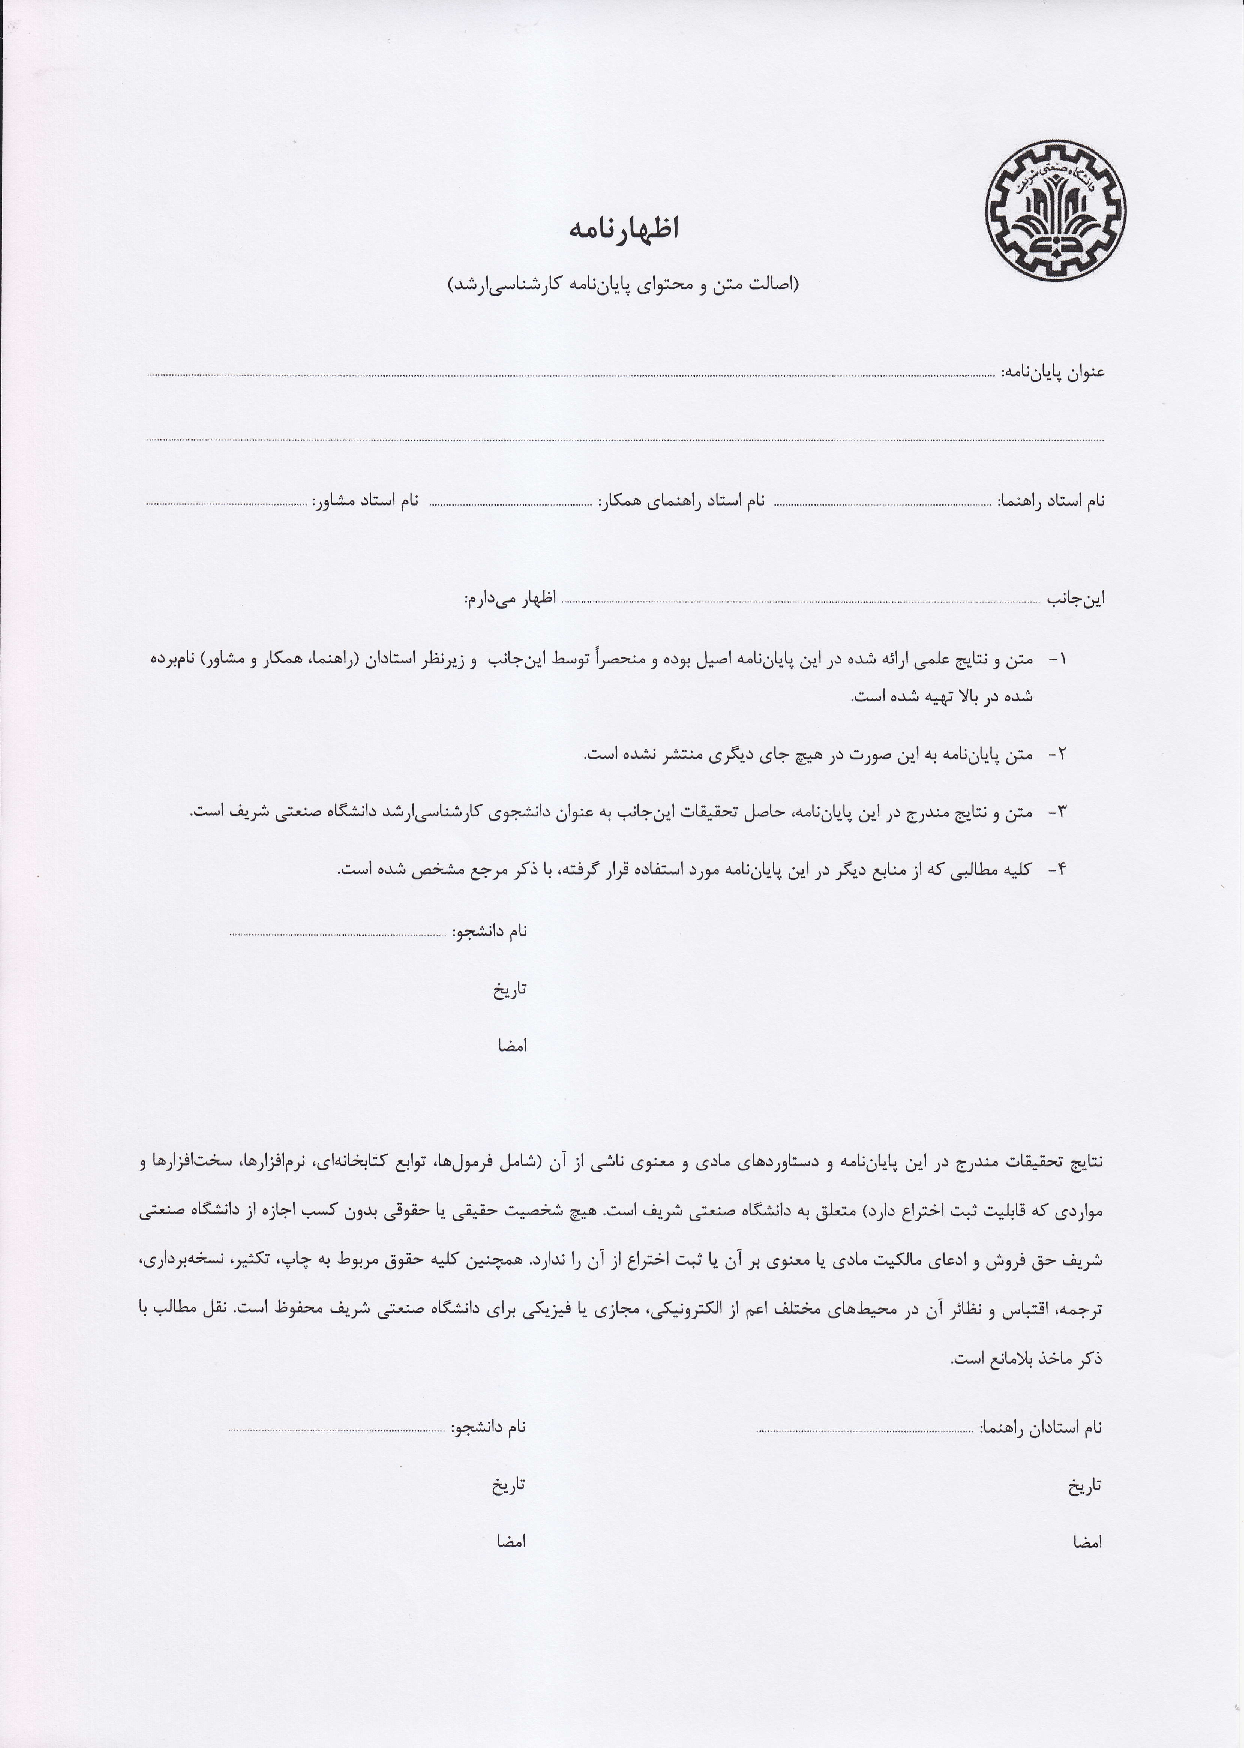
\includepdf[pages=-]{Esalat.pdf} % use scanned version for final steps!
		\thispagestyle{empty}
\begin{tabular}{m{0.15\textwidth} m{0.70\textwidth} m{0.15\textwidth}}
\multirow{2}{*}{
\includegraphics[width=2.5cm]{logo}}
 & 
\centering \Large{اظهارنامه} \normalsize & \\
 & \centering \large{(اصالت متن و محتوای پایان‌نامه کارشناسی‌ارشد)}   &  \\
\end{tabular}
\newline
\vspace{2cm}
\newline
عنوان پایان‌نامه:
\fatitle{}
\newline
\vspace{0.2cm}
\newline
نام استاد راهنما: 
\fasupervisor{} \hspace{.5cm}
نام استاد راهنمای هم‌کار: 
\fahamkar{} \hspace{.5cm}
نام استاد مشاور: 
\famoshaver{}
\newline\newline
این‌جانب 
\faAuthor{}
 اظهار می‌دارم:
\begin{enumerate}
\item
متن و نتایج علمی ارائه شده در این پایان‌نامه اصیل بوده و منحصرا توسط این‌جانب زیر نظر استادان (راهنما، همکار و مشاور) نام‌برده شده در بالا تهیه شده است.
\item
متن پایان‌نامه به این صورت در هیچ جای دیگری منتشر نشده است.
\item
متن و نتایج مندرج در این پایان‌نامه، حاصل تحقیقات این‌جانب به عنوان دانشجوی کارشناسی‌ارشد دانشگاه شریف است.
\item
کلیه مطالبی که از منابع دیگر در این پایان‌نامه مورد استفاده قرار گرفته، با ذکر منبع مشخص شده است.
\end{enumerate}
\begin{tabular}{m{0.55\textwidth} m{0.45\textwidth}}
	&
نام دانشجو: 	
\hspace{0.1cm} \faAuthor{}
\\ & 
تاریخ
\\ & 
امضا
\\
\end{tabular}
\newline\newline\newline\newline
نتایج تحقیقات مندرج در این پایان‌نامه و دستاوردهای مادی و معنوی ناشی از آن (شامل فرمول‌ها، توابع کتابخانه‌ای، نرم‌افزارها، سخت‌افزارها و مواردی که قابلیت ثبت اختراع دارد) متعلق به دانشگاه صنعتی شریف است. هیچ شخصیت حقیقی یا حقوقی بدون کسب اجازه از دانشگاه صنعتی شریف حق فروش و ادعای مالکیت مادی یا معنوی بر آن یا ثبت اختراع از آن را ندارد. همچنین کلیه حقوق مربوط به چاپ، تکثیر، نسخه‌برداری، ترجمه، اقتباس و نظائر آن در محیط‌های مختلف اعم از الکترونیکی، مجازی یا فیزیکی برای دانشگاه صنعتی شریف محفوظ است. نقل مطالب  با ذکر ماخذ بلامانع است.
\newline\newline
\begin{tabular}{m{0.07\textwidth} m{0.48\textwidth} m{0.45\textwidth}}
	&
	نام استاد راهنما: 
	\hspace{0.1cm} \fasupervisor{}
	&
	نام دانشجو: 	
	\hspace{0.1cm} \faAuthor{}
	\\
	&
	تاریخ
	& 
	تاریخ
	\\
	&
	امضا
	&
	امضا
	\\
\end{tabular}
		%\thispagestyle{empty}

{\nastaliq
 قدردانی

با تشکر از پدر، مادر و خواهر عزیزم به پاس حمایت‌ها و زحماتی که در این سال‌ها برای من کشیدند.   همچنین از سرکار خانم دکتر سلیمانی استاد راهنمایم به پاس راهنمایی‌های ارزشمندشان تشکر و قدردانی می‌کنم. 

همچنین از اساتید محترم جناب آقای دکتر صامتی و جناب آقای دکتر فاطمی‌زاده برای قبول زحمت داوری رساله و نظرات سازنده‌ی ایشان سپاسگزارم.

در نهایت از همراهی و همیاری اعضای آزمایشگاه یادگیری ماشین و همه‌ی دوستانم، تشکر می‌کنم. 
}\\[2cm]
\newpage\clearpage % use scanned version for final steps!
		\thispagestyle{empty}
\centerline{\textbf{\large{چکیده}}}
\begin{quote}
دنباله‌ها بخش زیادی از اطلاعات دنیای واقعی را تشکیل می‌دهند، که بارزترین نمونه‌ی آن زبان‌های طبیعی است. بسیاری از ساختارهای مهم نیز قابلیت مدل شدن به عنوان دنباله را داشته و داده‌هایی مثل ساختار مولکول، گراف و نت‌های موسیقی را نیز می‌توان به عنوان دنباله در نظر گرفت. از سوی دیگر تولید دنباله‌های جدید و بامعنی در هر حوزه، موضوعی با اهمیت و کاربردی است، مثلا در ترجمه‌ی زبان طبیعی یا کشف ساختار داروی جدید با ویژگی‌های خاص، مساله‌ی تولید دنباله وجود دارد.
با این وجود مشکلات مهم زیادی برای حل مساله‌ی تولید دنباله مطرح است، از جمله این مشکلات می‌توان به گسسته بودن جنس داده‌ها و انتخاب تابع هدف مناسب اشاره کرد. 
روش‌های پایه‌ی ارائه‌شده در این حوزه، دارای مشکلاتی نظیر اُریبی مواجهه میان زمان آموزش و آزمون و تابع هدف نامناسب هستند، از این رو نیاز به روش‌های جدید در این حوزه احساس می‌شود.
\newline  
در چند سال اخیر پیشرفت‌های زیادی در حوزه‌ی تولید تصویر  به وسیله‌ی شبکه‌های مولد مقابله‌ای انجام شده است. همین موضوع باعث شده که استفاده از شبکه‌های مولد مقابله‌ای در تولید دنباله‌ها نیز به تازگی مورد توجه قرار گیرد.  اما به دلیل گسسته بودن جنس دنباله‌ها، این امر به سادگی میسر نبوده و برای حل آن نیاز به استفاده از راهکار‌هایی مثل یادگیری تقویتی و استفاده از تقریب وجود دارد.
به علاوه ناپایداری شبکه‌های مولد مقابله‌ای باعث ایجاد چالش‌های جدید و زیاد شدن پیچیدگی مساله می‌شود.
\newline
در این پژوهش، با بیان رویکردی جدید و مبتنی بر ایده‌ی شبکه‌های مولد مقابله‌ای، به ارائه‌ی روشی برای حل مساله‌ی تولید دنباله با رویکردی تکرار شونده می‌پردازیم، به طوری که مدل در هر گام الگوریتم، با آموزش در مقابل نمونه‌های تولیدی خودش بهبود می‌یابد.
اساس روش پیشنهادی تخمین نسبت چگالی احتمال بوده و با این رویکرد روشی بدون مشکل دربرابر گسستگی دنباله‌ها ارائه شده است.
راهکار ارا‌‌ئه شده نسبت به روش‌های شبکه‌های مولد مقابله‌ای در حوزه‌ی دنباله، آموزشی پایدار‌تر دارد؛ هم‌چنین مشکل اُریبی مواجهه نیز در روش پیشنهادی وجود ندارد.
\newline
از آنجا که ارزیابی مدل‌های مولد خود چالشی مورد تحقیق است، در بخش دیگری از پایان‌نامه به بررسی معیارهای موجود پرداخته و با ارائه سه نحوه‌ی ارزیابی جدید، سعی در رفع مشکل معیار‌های موجود و بهره بردن از نتایج پژوهش‌های مربوط به حوزه‌ی تصویر داریم. روش‌های ارزیابی پیشنهادی برخلاف معیار‌های پیشین که فقط کیفیت نمونه‌ها را بررسی می‌کنند، همزمان به تنوع نمونه‌های تولیدی در کنار کیفیت اهمیت می‌دهند.
آزمایش‌های این پژوهش نشان‌دهنده‌ی برتری روش پیشنهادی در مقابل روش‌های پیشین است.


\vskip 1cm
\textbf{کلمات کلیدی:} \textiranic{
شبکه‌های مقابله‌ای، ایجاد دنباله، شبکه‌های عصبی، یادگیری عمیق
}
\end{quote}
		\thispagestyle{empty}
		\cleardoublepage %
		
		
		% Tables
		%=======================================================
		\cleardoublepage % terminates the current paragraph and page, the same way as a report document.
		\pagenumbering{harfi}
		\tableofcontents
		\cleardoublepage % terminates the current paragraph and page, the same way as a report document.
		\listoffigures
		%\listoftables
		\cleardoublepage % terminates the current paragraph and page, the same way as a report document.
		\listoftables
		%\listoftables
		\cleardoublepage % terminates the current paragraph and page, the same way as a report document.
		\pagenumbering{arabic} 
		
		% Chapters
		%=======================================================
		\chapter{مقدمه}\label{Chap:Chap1}
\minitoc
در این فصل ابتدا به معرفی مساله‌ی تولید دنباله می‌پردازیم، اهمیت و کاربرد‌های این مساله را مورد بررسی قرار می‌دهیم. پس از آن به صورت مختصر درباره‌ی یادگیری 
\trans{مقابله‌ای}{Adversarial}
و دلیل توجه به آن توضیحاتی می‌دهیم. سپس چالش‌هایی ذاتی مساله، چالش‌هایی که در روش‌های پایه برای حل مساله وجود داشته و چالش‌های ایجاد شده با استفاده از یادگیری مقابله‌ای بیان می‌شود و فصل حاضر را با تشریح ساختار پایان‌نامه و فصول مختلف آن به پایان می‌بریم.
\section{تعریف مساله}
\label{sec:chap1:definition}
در این پژوهش هدف تولید دنباله‌های گسسته با آموزش بر روی نمونه‌هایی که از این دنباله داریم است.
دنباله‌ی گسسته به معنی تعدادی متغیر گسته است که ترتیب دارند و گسسته بودن دنباله به این معنی است که هر مقدار دنباله مقادیر محدودی می‌گیرد. در این پژوهش داده‌ی گسسته از نوع 
\trans{دسته‌ای}{Categorical}
مدنظر است (در مقابل داده‌های عددی مثل مجموعه‌ی اعداد صحیح). در داده‌های دسته‌ای همه‌ی مقادیر ممکن هم‌فاصله است، از این رو معمولا این مقادیر به صورت بردار
\trans{یک-فعال}{One-hot}
کد می‌شوند. هر یک از این مقادیر در دنباله را کلمه می‌نامیم.
\newpage
برای مثال یک نمونه از دنباله‌ی گسسته به صورت زیر است:
\begin{equation*}
\underbrace{\clubsuit}_{\text{عنصر اول}}
 \diamondsuit \bigstar \clubsuit \clubsuit \heartsuit \spadesuit \heartsuit \bigstar \clubsuit \clubsuit \spadesuit \heartsuit \heartsuit,
\end{equation*}

که از چپ به راست ترتیب دارند، هر یک از عناصر یکی از مقادیر 
$\{ \clubsuit , \diamondsuit ,\bigstar , \spadesuit , \heartsuit \} $
را به خود گرفته است و میزان شباهت هر دو مقداری از این مجموعه با همدیگر مساوی است.
\section{اهمیت و کاربرد}
داده‌های زیادی را می‌توان با دنباله مدل کرد، از این رو موضوع تولید دنباله دامنه‌ی وسیعی را در بر می‌گیرد.
در ادامه با ذکر تعدادی از این حوزه‌ها برای آن کاربرد‌هایی ذکر می‌شود و اهمیت آن تشریح می‌شود.
\begin{itemize}
	\item 
	\textbf{ زبان طبیعی:}
زبان طبیعی را می‌توان	دنباله‌ای از کلمات و یا حروف درنظر گرفت، تولید زبان طبیعی در ترجمه‌ی متن، سیستم‌های پاسخگویی خودکار، خلاصه‌سازی متن، تولید عنوان برای تصاویر و غیره کاربرد دارد.
هر یک از این مثال‌ها خود حوزه‌ی پراهمیتی است که به صورت جداگانه مورد پژوهش هستند.
بهبود مساله‌ی تولید دنباله می‌تواند منجر به بهبود در کاربرد‌های ذکر شده شود. 
		\item 
		\textbf{ ساختار مولکولی:}
		ساختارهای مولکولی را می‌توان با رشته‌های به نام
		\lr{SMILES}
		بیان کرد
		\cite{weininger1988smiles}.
		این نحوه‌ی بیان اطلاعات هندسی ساختار مولکولی را در خود دارد. این رشته‌ها دارای قواعد گرامری هستند و لزوما هر رشته‌ای متناظر یک ساختار مولکولی نیست
		\cite{ORGAN}،
		از این رو نیاز به روش‌هایی احساس می‌شود که دنباله‌های معتبر با ویژگی‌های خواسته شده تولید کند. 
برای مثال اگر مدل برای یک داروی موردنظر ساختار‌های مولکولی ارائه دهد که ویژگی‌های خاصی را داشته باشند، فرایند تولید دارو‌های جدید و شخصی‌سازی شده ساده‌تر و اقتصادی‌تر می‌شود. مولکول‌ها فقط محدود به دارو نیستند و در حوزه‌ای مثل کشف مواد جدید هم این بحث‌ وجود دارد
		\cite{ORGAN}.
		\item 
		\textbf{ گراف :}
		به تازگی روش‌هایی بر مبنای
\trans{گشت‌زنی تصادفی}{Random Walk}
در حوزه‌ی گراف ارائه شده است که نتایج موفقی داشته‌اند.
 در این روش بجای کار روی ساختار گراف بر روی دنباله‌های حاصل از گشت‌زنی تصادفی روی گراف کار می‌شود. 
برای تولید گراف، دنباله‌هایی به عنوان گشت‌زنی تصادفی آن تولید می‌شود و از روی این دنباله‌ها گراف ساخته می‌شود.
موضوع تولید گراف شامل حوزه‌های کاربرد‌های زیادی می‌شود، برای مثال در تولید
\trans{گراف دانش}{Knowledge Graph}
و یا گراف ساختار مولکولی کاربرد دارد
		\cite{Aleksandar18NetGAN, Jiaxuan18GraphRNN}.
		
		\item 
		\textbf{ موسیقی:}
				یکی از راه‌های ذخیره‌سازی باکیفیت موسیقی ثبت نُت‌های آن است، از آنجا که این نت‌ها تعداد حالات محدودی دارند و در زمان ترتیب دارند می‌توان آن را به عنوان‌ دنباله‌هایی در طول زمان مدل کرد
				\cite{SeqGAN}.
\end{itemize}


\section{يادگیری مقابله‌ای}
\label{Method:GAN:Shalow}
\trans{شبکه‌های مولد مقابله‌ای}{Generative Adversarial Networks}
\cite{Goodfellow2014}
روشی برای آموزش مدل 
\trans{مولد}{Generative}
 است بر این مبنا که شبکه‌هایی با هم رقابت می‌کنند و به نوعی با هم بازی انجام می‌دهند؛ نتیجه‌ی این رقابت آموزش مدل مولد است.
روش‌های آموزش مبتنی بر این ایده را یادگیری مقابله‌ای می‌نامیم.
در ادامه به نحوه‌ی کار روش شبکه‌های مولد مقابله‌ای معرفی شده در
\cite{Goodfellow2014}
می‌پردازیم و سپس چند دلیل برای اهمیت یادگیری مقابله‌ای‌ ذکر می‌کنیم.
\newline
در شبکه‌های مولد مقابله‌ای برای آموزش مدل مولد از شبکه‌ی دومی به عنوان
\trans{تمیزدهنده}{Discriminator}
استفاده می‌شود، این شبکه‌ یک
\trans{دسته‌بند}{Classifier}
دو دسته‌ای است. روال آموزش به این صورت است که تمیزدهنده بین دو مجموعه داده‌ی واقعی و داده‌های تولید شده توسط مولد دسته‌بندی انجام می‌دهد، سپس شبکه‌ی مولد به سمتی سوق داده می‌شود که تمیزدهنده را به اشتباه بیاندازد و این دو مرحله به صورت تکراری انجام می‌شود.
 در این روش آموزش تمیزدهنده مشابه یک دسته‌بند عادی انجام می‌شود.
 از آنجا که شبکه‌ی تمیزدهنده نسبت به ورودی مشتق‌پذیر است برای آموزش مدل مولد، گرادیان از شبکه‌ی تمیزدهنده وارد شده و پارامتر‌های مدل مولد را به‌روزرسانی می‌کند، به عبارت دیگر شبکه‌ی تمیزدهنده مشابه تابع هزینه برای مولد عمل کرده و مشخص می‌کند با تغییر پارامتر‌های مولد در چه راستایی تمیزدهنده به اشتباه می‌افتد.
\subsection{دلیل توجه به یادگیری مولدمقابله‌ای}
برای حل مساله‌ی تولید دنباله توجه زیادی به آموزش مقابله‌ای شده است
\cite{kusner2016gans,lamb2016professor,Zhang2017TextGAN,SeqGAN,ORGAN,lin2017adversarial,Guo2018,Che2017,press2017langwasserstein}،
در ادامه دلایلی برای این موضوع ذکر می‌کنیم.
	\begin{figure}[!htb]
		{
			\begin{center}
				\subfigure[تصاویر مصنوعی تولید شده]{\label{Figure:NVIDIAGAN:Sample}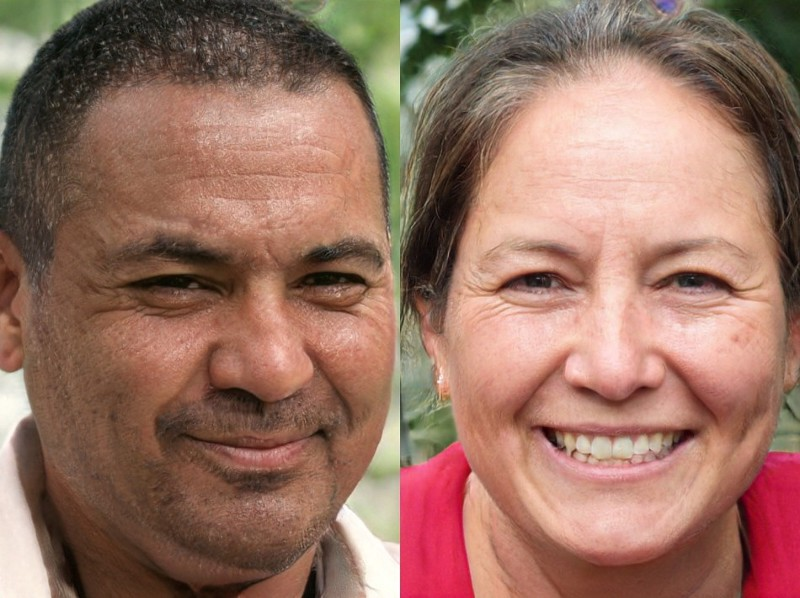
\includegraphics[scale=0.25]{images/Nvidia/SelectedGenerated.png}}
				\hspace{1cm}
				\subfigure[
				ادغام تصاویر در فضای ویژگی و تبدیل تصاویر مبدا به سبک تصویر مقصد
				]{\label{Figure:NvidiaGAN:Latent}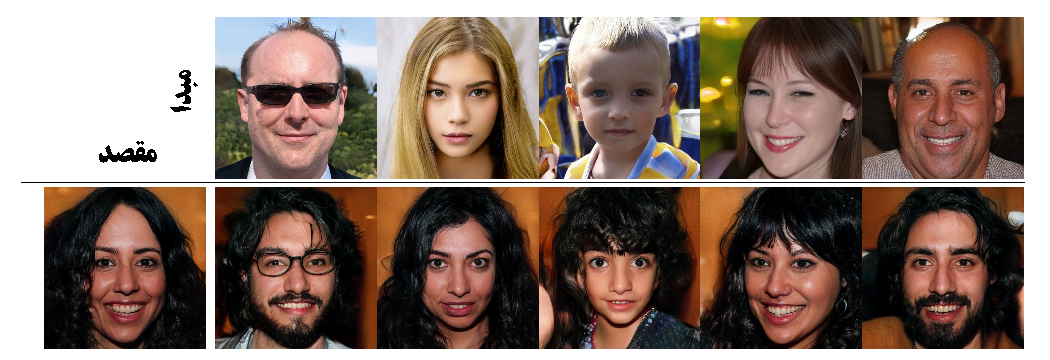
\includegraphics[scale=0.8]{images/Nvidia/SelectedStyle2.pdf}} 
				\end{center}
			\caption[نتایج یکی از آخرین پژوهش‌های انجام شده در حوزه‌ی تصویر با کمک شبکه‌های مولد مقابله‌ای]{
				نتایج یکی از آخرین پژوهش‌های انجام شده در حوزه‌ی تصویر با کمک شبکه‌های مولد مقابله‌ای
				\cite{karras2018style}
			}
			\label{Figure:NVIDIAGAN:SampleAndLatent}
		}
		\end{figure}

\begin{itemize}
	\item 
	\textbf{پیشرفت‌های چشم‌گیر یادگیری مقابله‌ای در حوزه‌ی تصویر:}
	بعد از معرفی یادگیری مقابله‌ای، این روش در حوزه‌ی تولید تصویر نتایج
	\trans{مرز دانش}{State-of-the-Art}
	را کسب کرده است و هر روزه شاهد پیشرفت‌های بیشتری در این حوزه با کمک یادگیری مقابله‌ای هستیم.
	\newline
	برای مثال در یکی از جدیدترین پژوهش‌هایی که توسط یک شرکت بزرگ ساخت کارت‌های گرافیکی بر روی تولید تصویر صورت انسان انجام شده است
	\cite{karras2018style}،
نتیجه‌ی این پژوهش علاوه بر کسب امتیاز بالایی در معیار ارزیابی مربوط به آن حوزه، موفق به تولید تصاویر بسیار نزدیک به تصاویر واقعی شده است.
به طوری که نمونه‌های ارائه شده در مقاله بسیار باکیفیت هستند و مصنوعی بودن آن غیرقابل تشخیص است، در شکل 
	\ref{Figure:NVIDIAGAN:Sample}
	دو نمونه از این تصاویر نمایش داده شده است. به علاوه فضای
	\trans{نهان}{Latent}
	که بر روی تصاویر صورت به دست آمده با معنی بوده و قابلیت ترکیب تصاویر تولید شده را می‌دهد، برای مثال شکل
	\ref{Figure:NvidiaGAN:Latent}
	نشان دهنده‌ی چند تصویر ورودی در سطر اول است که با کمک فضای ویژگی به دست آمده، به
	\trans{سبک}{Style}
	تصویر سمت چپ تبدیل شده‌اند. به این ترتیب، به واسطه‌ی عملکرد مناسب این روش‌ها در حوزه‌ی تولید تصویر، در دو سال اخیر توجه به سمت استفاده از مدل‌های مولدمقابله‌ای در حوزه‌ی تولید متن هم جلب شده است.
	\item 
	\textbf{قابلیت استفاده از دسته‌ی بزرگی از فاصله‌ها: }
	اثبات شده است که آموزش به وسیله‌ی شبکه‌های مولد مقابله‌ای،
 معادل کاهش فاصله‌ی
\lr{Jensen-Shannon}
بین توزیع اصلی و توزیع مولد است
\cite{Goodfellow2014}.
هم‌چنین روش‌های مبتنی بر یادگیری مقابله‌ای برای کاهش فاصله‌های دیگر هم پیشنهاد شده است
\cite{Nowozin2016, Poole2016}.
این فاصله‌ها روش مستقیم برای استفاده به عنوان
\trans{تابع هزینه‌}{Cost Function}
  ندارند و این امر با کمک یادگیری مقابله‌ای محقق شده است.
	\item 
	\textbf{کمک به حل بعضی مشکلات موجود در روش‌های پایه:}
	در روش‌های پایه‌ی تولید دنباله مشکلاتی مثل
 \trans{اُریبی مواجهه}{Exposure Bias}
	وجود دارد که دلیل آن رفتار متفاوت مولد در دو فاز 
\trans{آموزش}{Train}
	 و 
\trans{آزمون}{Test}
	 است. در ادامه در بخش چالش‌ها بیشتر به این موضوع می‌پردازیم.
 معمولا روش یادگیری مقابله‌ای دچار این مشکل نمی‌شوند، زیرا اکثر این روش‌ها فاز آموزش و آزمون یکسانی برای تولید دنباله دارند.
\end{itemize}

\section{چالش‌ها}\label{ch1:dooshvari}
در این بخش ابتدا به چالش معیار ارزیابی و تابع هزینه که چالش ذاتی مساله است می‌پردازیم، در ادامه نمونه‌ای از مشکل روش پایه را بیان کرده و در پایان مشکلات استفاده از یادگیری مقابله‌ای را در مساله بیان می‌کنیم.
\subsection{مشخص نبودن معیار ارزیابی مناسب}
در حوزه‌ی مدل‌های مولد معیار ارزیابی مشخصی وجود ندارد و نحوه‌ی ارزیابی این مدل‌ها خود یک چالش است
\cite{Lucas15NoteOnEvaluation}.
ارزیابی مدل‌های مولد دنباله هم از این قاعده مستثنی نیست و معیاری استانداردی به جز قضاوت انسانی وجود ندارد. به دلیل اهمیت معیار ارزیابی، فصل
\ref{Chap:Chap4}
به این موضوع اختصاص داده‌شده است.
\subsection{مشخص نبودن تابع هزینه مناسب}
مشکلی مشابه در حوزه‌ی انتخاب تابع هزینه مورد استفاده وجود دارد و بخش عمده‌ای از پژوهش‌های انجام شده در حوزه‌ی تولید دنباله به روش‌های آموزش و تابع‌های هزینه اختصاص دارد.
\newline
\trans{تابع هدف}{Objective Function}
اولیه مورد استفاده در روش‌های پایه مبتنی بر  
\trans{بیشینه درست‌نمایی}{Maximum Likelihood}
است. این تابع هدف به این معنی است که در آموزش مدل، هدف افزایش احتمالی است که مدل به داده‌های آموزش می‌دهد و به سمتی می‌رود که از دید مدل، داده‌های واقعی احتمال بالایی بگیرند؛
ولی اینکه به دنبال مدل‌هایی باشیم که نمونه‌های تولیدی آن در توزیع واقعی داده‌ها (که در دسترس نیست) احتمال بالایی بگیرند، رویکرد منطقی‌تری است. با این وجود راه‌حلی برای استفاده از این تابع هدف وجود ندارد.
روش‌های یادگیری مقابله می‌توانند استفاده از تابع هدف‌های بهتر را ممکن کنند
\cite{Huszar15HowNot}.
درست‌نمایی مدل را به سمتی می‌برد که به داده‌های آموزش احتمال بالایی دهد، ولی این موضوع را کمتر در نظر می‌گیرد که به نمونه‌های غیر از داده‌های آموزش احتمال کمی نسبت دهد. این ویژگی می‌تواند منجر به رفتاری شود که به نمونه‌ی نامعتبری احتمال بالا نسبت داده شود، این رفتار به نام 
 \trans{میانگین-جستجوگری}{Mean-Seeking}
شناخته می‌شود که در
ادامه بیشتر توضیح داده شده است.
 \subsubsection{رفتار میانگین-جستجوگری}
 در حالتی که ظرفیت مدل به اندازه‌ی کافی است با در نظر گرفتن تابع درست‌نمایی به عنوان تابع هدف می‌توان توزیع داده‌ی اصلی را یاد گرفت. 
 ولی در حالتی که ظرفیت مدل در مقابل داده‌های آموزش کم است مدل نمی‌تواند توزیع اصلی را کاملا یاد بگیرد و بسته به تابع‌ هزینه رفتار‌های متفاوتی را بروز می‌دهد. رفتاری که با تابع هدف درست نمایی بروز داده می‌شود باعث می‌شود توزیع آموزش دیده کل توزیع داده اصلی را در بر بگیرد و در این بین ممکن است به نقاطی از فضا بیشترین احتمال را نسبت دهد که دادها‌ی اصلی در آنجا احتمال کمی دارند. 
 این رفتار میانگین-جستجوگری نامیده می‌شود.
 در حوزه‌ی مدل‌های مولد این رفتار به این معنی است که مدل می‌خواهد داده‌هایی شبیه به تمام داده‌های آموزش تولید کند، حتی به این قیمت که بعضی از داده‌های تولیدی شبیه به داده‌های آموزش نباشد
 \cite{Huszar15HowNot}.
 به صورت کلی‌تر رفتار میانگین-جستجوگری مربوط به استفاده فاصله‌ی 
\lr{Kullback-Leibler (KL)}
 بین توزیع داده اصلی و توزیع مدل به عنوان تابع هزینه است، در ادامه دلیل این رفتار بیان شده است.
  \begin{figure}[!htb]
  	{
  		\begin{center}
  			\subfigure[ بیشینه درست‌نمایی]{\label{Figure:MLE:MLEvsReverseKL:KL}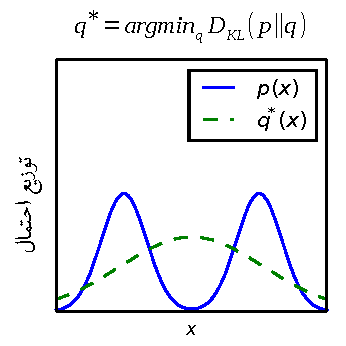
\includegraphics[scale=1]{images/KLvsReverseKL_KL.pdf}}
  			\hspace{1cm}
  			\subfigure[معکوس فاصله‌ی \lr{KL}]{\label{Figure:MLE:MLEvsReverseKL:ReverseKL}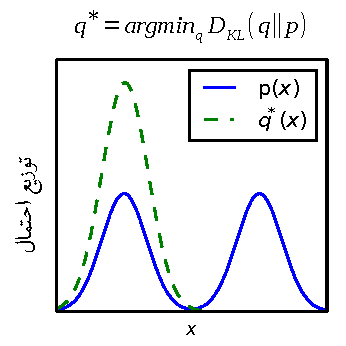
\includegraphics[scale=1]{images/KLvsReverseKL_RKL.pdf}} 
  		\end{center}
  		\caption{مقایسه رفتار بیشینه درست‌نمایی و معکوس فاصله‌ی}
  		\label{Figure:MLE:MLEvsReverseKL}
  	}
  \end{figure}
 \newline
 برای توجیه رفتار میانگین-جستجوگری، حالتی را در نظر بگیرید که این رفتار رخ ندهد یعنی محلی در فضا توزیع احتمال داده‌ی اصلی مقدار دارد و توزیع مدل به آن نقطه احتمال صفر نسبت داده است، در این شرایط تابع هزینه به سمت بی‌نهایت می‌رود و بنابر این در آموزش از چنین حالتی دوری می‌شود و هر نقطه از فضای داده که احتمال دارد، باید مدل هم احتمالی به آن نقطه نسبت دهد.
 \newline
 به عنوان یک مثالی از این رفتار، اگر فرض کنیم داده‌های واقعی توزیع دو قله‌ای گاوسی دارند و خانواده‌ی مدل مولدی که درنظر گرفته‌ایم گاوسی تک قله‌ای باشد، در شکل 
 \ref{Figure:MLE:MLEvsReverseKL:KL}
نتیجه آموزش با شرایط گفته شده نشان داده شده است، که 
 $p(x)$ 
 توزیع واقعی داده‌ها و
 $q^\star(x)$
 بهینه است. نتیجه آموزش با درست نمایی در این حالت باعث شده مدل به نقطه‌ای از فضا احتمال زیادی دهد که داده‌های اصلی احتمال کمی دارند. شکل 
 \ref{Figure:MLE:MLEvsReverseKL:ReverseKL}
 حالتی است که معکوس فاصله‌ی
 \lr{KL}
 کمینه شده و به سمتی رفته که یکی از قله‌های توزیع اصلی را یاد بگیرد که از یک جهت رفتار مناسب‌تری است. به عبارت دیگر این حالت باعث تولید نمونه‌ی نامعتبر نمی‌شود ولی می‌تواند تنوع در نمونه‌های تولیدشده را محدود کند.
\subsection{ناهماهنگی آموزش و آزمون}\label{sec1:exposurebias}
در برخی از روش‌ها نمی‌توان رفتار مشابه در آموزش و آزمون داشت که این مساله باعث می‌شود که خطایی در آموزش ایجاد شود. در ادامه به ذکر یک نمونه از این مشکل می‌پردازیم.
\newline
در اکثر روش‌ها برای تولید دنباله، مساله ساده‌سازی می‌شود و به این شکل تبدیل می‌شود که با داشتن یک زیردنباله عنصر بعدی دنباله چگونه باید باشد. 
بنابراین اگر در گام آموزش این زیردنباله‌ها فقط داده‌های واقعی باشند مشکل 
\trans{ناهماهنگی}{Inconsistency}
آموزش و آزمون پیش می‌آید، زیرا مدل فقط تصمیم گیری با دنباله‌های کاملا صحیح را آموزش دیده ولی در گام آزمون با زیردنباله‌های تولید خودش مواجه می‌شود، این مشکل اُریبی مواجهه نامیده می‌شود.
\subsection{مشکل انتقال گرادیان } \label{Problem:GradientPass}
راهکارهای زیادی برای استفاده از یادگیری مقابله‌ای در حوزه‌ی داده‌های پیوسته پیشنهاد و استفاده شده است، ولی به دلیل مشکل انتقال گرادیان در داده‌های گسسته، مستقیما امکان استفاده از این روش‌ها در حوزه‌ی داده‌های گسسته وجود ندارد.
\newline
روش بهینه‌سازیی که برای آموزش شبکه‌های عصبی استفاده می‌شود مبتنی بر محاسبه‌ی گرادیان نسبت به پارامترهای شبکه است و روش‌های یادگیری مقابله‌ای هم نیازمند محاسبه‌ی این گرادیان هستند.
برای به‌روز‌رسانی شبکه مولد لازم است که نمونه‌‌های تولید شده توسط شبکه‌ی مولد وارد دسته‌بند شده، سپس با کمک دسته‌بند تغییر پارامتر‌های شبکه‌ی مولد در جهتی که شبکه‌ی دسته‌بند فریب بخورد (یا همان گرادیان)، محاسبه ‌شود. 
برای اینکه گرادیان نسبت به پارامتر‌های شبکه‌ی مولد قابل محاسبه باشد، باید تمام عملیات ایجاد نمونه و محاسبه‌ی خروجی دسته‌بند دارای مشتق تعریف شده باشند.
\newline
در مساله‌ی تولید دنباله معمولا در انتهای شبکه‌ی مولد نیاز به نمونه‌گیری از یک توزیع است، این عملیات مشتق تعریف شده‌ای ندارد که این موضوع باعث بروز مشکل انتقال گرادیان می‌شود
\cite{SeqGAN}.
مشکل انتقال گرایان به معنی عدم توانایی انتقال گرادیان تولید شده توسط دسته‌بند به شبکه‌ی مولد است.
این چالش تنها مربوط به حوزه‌ی یادگیری مقابله‌ای نبوده و برای تقریب گرادیان پژوهش‌هایی مثل
\cite{JanGuPoo17}
انجام شده است.
در ادامه دلایل این مشکل با جزئیات بیشتر تشریح شده است.
\subsubsection{تعریف نشده بودن مشتق عملیات تصادفی}
زمانی که متغیر تصادفی $z$ تابعی از $\theta$ است و این رابطه تصادفی است، در حالت کلی مشتق $z$ نسبت به $\theta$ تعریف نشده است. این مشکل در
\trans{خود رمزگذار وردشی}{Variational Autoencoder}
هم وجود داشته و راه حل
\trans{تنظیم مجدد}{Reparametrization}
برای آن پیشنهاد شده است
\cite{JanGuPoo17}.
\newline
 برای مثال، یک نمونه استفاده از این تکنیک در رابطه با توزیع گوسی است، فرض کنید متغیر تصادفی $z$ به طوری تعریف می‌شود که
$z \sim N(f_\theta,1)$
باشد، در حالت عادی مشتق $z$ به پارامتر $\theta$ تعریف نشده است ولی با بازنویسی $z$ به صورت
$f_\theta + N(0,1)$
مشکل حل شده و با حذف قسمت تصادفی از مسیر تبدیل $\theta$ به $z$ مشتق تعریف شده است. متاسفانه در شبکه‌های مولد مقابله‌ای برای تولید دنباله، این مشکل به راحتی قابل حل نیست.
 در بخش
\ref{Method:GumbelSoftmax}
توضیحات بیشتری در این رابطه بیان شده است.
\subsubsection{گسسته بودن خروجی شبکه}
مشکل عدم وجود مشتق در مثال گاوسی به این دلیل قابل حل بوده که بعد از تکنیک تنظیم مجدد در مسیر تبدیل $\theta$ به $z$ تمام عملیات مشتق‌پذیر است.
در حالی که در تولید دنباله گسستگی مقادیر، تعریف دقیق مشتق را ناممکن می‌کند و تنها راه‌کارهای تقریبی ممکن هستند. شبکه‌ا‌ی که در مساله‌ی تولید دنباله گسسته استفاده می‌شود نیازمند تولید داده‌های گسسته است و بنابراین خروجی شبکه‌ی مولد نوع گسسته دارد.
\newline
مشکل گسسته بودن خروجی عملیات را از دو دیدگاه می‌توان بیان کرد.
دیدگاه اول اینکه برای مشتق این عملیات راه حلی نداریم و راه عملی برای انجام آن وجود ندارد. برای مثال در نظر بگیرید رابطه‌ی 
${z = \argmax_i f_i(\theta)}$
برای $z$ برقرار است و می‌خواهیم مشتق $z$ نسبت به $\theta$ را محاسبه کنیم که روش برای آن نداریم.
دیدگاه دوم به صورت بررسی هندسی است، فرض کنید تابع $f$ به صورت 
${z=f(\theta)}$
تعریف شده است و خروجی آن گسسته است، یعنی $z$ دارای $N$ حالت ممکن است. فضایی که پارامتر‌های 
$\theta$
می‌سازند را در نظر بگیرید، از آنجا که در کل $N$ حالت خروجی وجود دارد، بنابراین فضای پارامتر‌های $\theta$ به $N$ بخش افراز می‌شود. اگر $\theta$ نقطه‌ای در یکی از نواحی فضا باشد با تغییرات محلی در مقدار $\theta$ خروجی تغییری نمی‌کند و مشتق معنی ندارد
\cite{SeqGAN}
، شکل 
\ref{Figure:DiscreteSpace}
توصیفی از چنین فضایی است.
\begin{figure}[!htb]
	\centering
	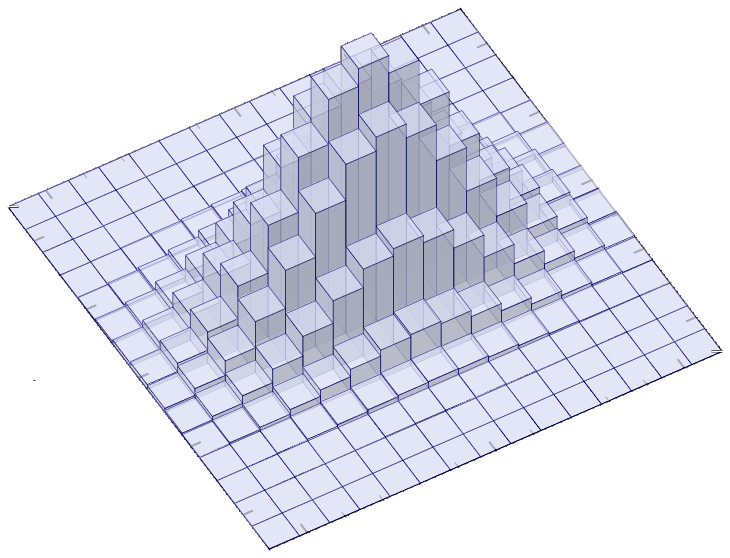
\includegraphics[width=0.5\textwidth]{images/DiscreteSpace.png} 
	\caption[ نمایش یک نمونه تابع از مقدار پیوسته‌ی دو بعدی به یک مقدار گسسته]
	{
		نمایش یک نمونه تابع از مقدار پیوسته‌ی دو بعدی به یک مقدار گسسته، در چنین فضایی روش‌های مبتنی بر گرادیان برای پیدا کردن نقطه‌ی بیشینه کارساز نیست.
	}
	\label{Figure:DiscreteSpace}
\end{figure}
\subsection{ناپایداری آموزش مقابله‌ای} \label{Problem:GANinstablity}
 	\begin{figure}[!htb]
 		{
 			\begin{center}
 				\subfigure[آموزش ناپایدار]{\label{Figure:GANInstability:Bad}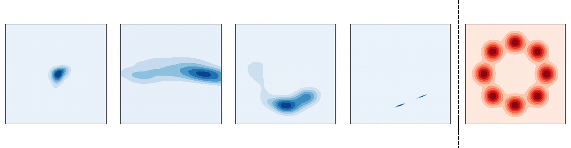
\includegraphics[scale=1.1]{images/GANBadTrain.pdf}}
 				\hspace{1cm}
 				\subfigure[آموزش پایدار]{\label{Figure:GANInstability:Good}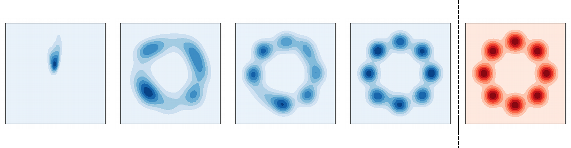
\includegraphics[scale=1.1]{images/GANGoodTrain.pdf}} 
 				\end{center}
 			\caption[نمایش ناپایداری آموزش شبکه‌های مولد مقابله‌ای و پایدارکردن آن ]{
 				نمایش ناپایداری آموزش شبکه‌های مولد مقابله‌ای و پایدارکردن آن با روش معرفی شده در
 				\cite{Mescheder17TheNumericOfGan}.
 				تصویر سمت راست توزیع داده‌ی اصلی را نشان می‌دهد و بقیه تصاویر از چپ به راست توزیع مدل مولد در حین آموزش و در گام‌های ۰، ۵۰۰۰، ۱۰۰۰۰ و ۲۰۰۰۰ آموزش است.
 			}
 			\label{Figure:GANInstability:BadAndGood}
 		}
 		\end{figure}
بزرگترین چالشی که در روش‌های آموزش مقابله‌ای وجود دارد ناپایداری آموزش آن است.
دو نمونه‌ از این ناپایداری به شرح زیر است:
\begin{itemize}
	\item 
آموزش مقابله‌ای می‌تواند به رفتار ناپایداری منجر شود که توزیع مدل مولد بین چند قله از توزیع اصلی به صورت تناوبی جابجا شود که این رفتار
 \trans{چسبیدگی به قله}{Mode Collapsing}
 نام دارد.
 یک مثال از چسبیدگی به قله در شکل
 \ref{Figure:GANInstability:Bad}
 نشان داده شده است و نشان می‌دهد که در آموزش یک توزیع چندقله‌ای به عنوان توزیع اصلی، مدل مولد بین قله‌ها به صورت تناوبی جابجا می‌شود.
 هم‌چنین شکل
 \ref{Figure:GANInstability:Good}
 نشان دهنده‌ی حالتی است که با تکنیک معرفی شده در
 \cite{Mescheder17TheNumericOfGan}،
 این آموزش پایدار شده است.
 \item
 مشکل دیگر در تکنیک مطرح‌شده در تنظیم نسبت آموزش مدل‌ مولد و تمیزدهنده است. به این صورت که اگر مدل تمیزدهنده به خوبی آموزش ببیند تمام نمونه‌های مدل مولد را به راحتی تشخیص می‌دهد و این موضوع باعث سخت شدن آموزش مولد می‌شود. مثلا فرض کنید شبکه‌ی مولد بر اساس امتیازی که از تمیزدهنده می‌گیرد آموزش می‌بیند و در حالتی که تمیزدهنده خیلی قویتر باشد به همه‌ی حرکت‌های خوب مولد امتیاز بسیار کوچکی می‌دهد که این موضوع باعث آموزش ندیدن مولد در عمل می‌شود. در واقع نزدیک نقطه‌ی بهینه برای تمیزدهنده، گرادیان نزدیک صفر است و چندان نمی‌تواند به بهبود مولد کمک کند.
\end{itemize}
 برای پایدار کردن آموزش روش‌هایی ارائه شده است
 \cite{Arjovsky17Wasserstein, Gulrajaniy17ImprovedWasserstein, Mescheder17TheNumericOfGan, Roth18StabilizeGAN, Luke16UnrolledGAN,Salimans16ImprovedTechTrainingGAN}،
 ولی بسیاری از این روش‌ها خاص حوزه‌ی داده‌های پیوسته است و نمی‌توان از آنها در تولید دنباله مستقیما بهره برد.
\section{هدف پژوهش}
با توجه به تعریف مساله در بخش 
\ref{sec:chap1:definition}
و چالش‌هایی که برای حل آن وجود دارد، در ادامه قصد داریم روشی برای تولید دنباله ارائه کنیم که بر پایه‌ی شبکه‌های مولد مقابله‌ای است، اما با مشکلاتی نظیر انتقال گرادیان رو به رو نیست. هم‌چنین در جهت ارزیابی موثرتر مدل پیشنهادی، معیارهای سنجش کیفیت را مورد مطالعه‌ی دقیق قرار داده و معیارهای جدیدی را برای این منظور پیشنهاد می‌کنیم.

\section{ساختار پایان‌نامه}
در ادامه‌ی مستند حاضر، در فصل دوم به تشریح کار‌های پیشین در زمینه‌ی تولید دنباله می‌پردازیم و با بررسی مزایا و معایب این روش‌ها، رویکردهای مختلف حل این مساله را با یکدیگر مقایسه می‌کنیم و در فصل سوم راهکار پیشنهادی برای تولید دنباله را معرفی می‌کنیم.
از آنجا که معیار ارزیابی خود موضع چالش برانگیزی در این حوزه است فصل چهار را به تشریح این معیارها می‌پردازیم و معیارهای جدیدی را پیشنهاد می‌کنیم. با ارائه آزمایش‌های انجام شده در فصل پنجم، به ارزیابی روش پیشنهادی می‌پردازیم. در نهایت با جمع‌بندی مطالب ارائه شده و ارائه پیشنهاداتی برای ادامه پژوهش، پایان‌نامه را به پایان می‌بریم.




		\chapter{پژوهش‌های پیشین}\label{Chap:Chap2}
\minitoc
		\chapter{راهکار پیشنهادی}\label{Chap:Chap3}
\minitoc
		\chapter{ معیارهای ارزیابی پیشین و پیشنهادی}\label{Chap:Chap4}
\minitoc

		\chapter{ارزیابی}\label{Chap:Chap5}
\minitoc
		\chapter{جمع‌بندی و کار‌های آتی}\label{Chap:Chap6}
\minitoc
در این پژوهش  جدیدترین کار‌های پیشین در حوزه‌ی تولید دنباله مورد بررسی قرار گرفت و  برخی از مزایا و معایب آنها بررسی شد. معیار‌هایی که روش‌های گذشته برای اثبات بهبودهای خود استفاده کرده‌اند، مورد نقد و بررسی قرار گرفت و مشاهده شد که  معیارهای مورد استفاده در برخی از روش‌ها، قضاوت ناعادلانه‌ای را انجام داده‌اند.
این مشکل  ریشه در ارزیابی کیفیت نمونه‌های تولیدی  بدون توجه به تنوع آنها دارد.
از این رو چند معیار جدید برای رفع این مشکل بیان و آزمایش‌هایی بر مبنای این معیارها انجام شد.
در آزمایش‌ها، کیفیت بالا و تنوع کم نتایج روش‌های مبتنی بر شبکه‌های مولد مقابله‌ای نشان داده شد و به این جمع‌بندی رسیدیم که روش‌های پیشین بر اساس یادگیری  مقابله‌ای در معیار‌هایی که همزمان کیفیت و تنوع را ارزیابی می‌کنند، پیشرفتی نسبت به روش پایه‌ی جبر معلم نداشته‌اند.
به علاوه ناپایداری این روش‌ها در آموزش نشان داده شد، این موضوع خود می‌تواند دلیلی بر نتایج نامناسب این دسته از روش‌ها باشد.


روش پیشنهادی با ایده‌ی آموزش  مولد توسط تمیزدهنده، بر مبنای تخمین نسبت چگالی دو توزیع معرفی و دو رویکرد برای این روش تشریح شد.
هم‌گرایی هر دو رویکرد به شکل نظری مورد بررسی قرار گرفت. هم‌چنین دیدیم که رویکرد اول در آزمایش‌ها نتایج بهتری نسبت به دیگر روش‌ها کسب کرد و نشان داد که آموزش پایداری دارد. از سوی دیگر، رویکرد دوم به صورت نظری دقیق‌تر بررسی شد و نشان داده شد که با در نظر گرفتن فرض سبکی برای تمیزدهنده، در هر گام مولد بهبود اتفاق می‌افتد.


برای کارهای آینده، در سه مسیر می‌توان پژوهش را ادامه داد.
\newline
مسیر اول، بررسی معیار‌های پیشنهادی و معیار‌های موجود است.
این بررسی‌ها می‌تواند شامل بررسی  مقاومت و حساسیت معیار  باشد. برای نمونه، نیاز به بررسی تغییر معیار در مقابل تخریب دنباله‌ها است. هم‌چنین حساسیت معیار به نحو و یا معنای دنباله‌ها و بخصوص دنباله‌های زبان طبیعی جای بررسی بیشتر دارد. هم‌چنین بررسی‌های دیگری مثل اثر طول دنباله بر معیارها نیازمند مطالعه است.
\newline
مسیر دوم، بررسی بیش‌تر روش پیشنهادی از نظر عملی است. اینکه چه ساختار‌هایی مناسب شبکه‌ی تمیزدهنده است و هم‌چنین نحوه‌ی تاثیر تابع
$f$
انتخابی در تابع هزینه (که در تحلیل نظری روش گفته شد) در عمل چگونه است. به‌علاوه تعمیم روش به حالتی که هدف، تولید دنباله‌هایی  به صورت شرطی باشد نیز می‌تواند مورد بررسی قرار بگیرد.
\newline
مسیر سوم، بهبود روش‌های پیشین است. زیرا در  این پژوهش با مشکلاتی در روش‌های پیشین مواجه شدیم که مورد توجه نبوده است. 
امید می‌رود که حل این مشکلات موجب بهبود روش‌های پیشین در حوزه باشد. برای مثال روش
\lr{SegGAN}
از جستجوی مونت کارلو برای تخمین امتیاز زیر دنباله‌ها استفاده می‌کند، انتظار داریم بتوان مشابه روش پیشنهادی، با شبکه‌ای بازگردنده این تخمین مستقیما محاسبه شود. به عنوان نمونه‌ای دیگر، متوجه شدیم که در روش‌های یادگیری مقابله‌ای با رویکرد تولید دنباله‌ی «توزیع کلمه» (بخش 
\ref{Ch2:Section:Method:SequenceOfDistribution})،
اُریبی وجود دارد. این اُریبی در تفاوت آموزش و آزمون است. زیرا این روش‌ها در آموزش توزیع را تولید می‌کنند ولی در آزمون از 
$\argmax$
توزیع تولیدی را برای تولید دنباله استفاده می‌کنند. امید می‌رود با استفاده از تکنیک‌های مشابه
\lr{Gumbel Softmax}
این اُریب رفع شود.



		% Appendices, Glossaries and Refrences
		%=======================================================
		\begin{appendices}
			%\resettranslations % reset the first-use flag of tranlsation glossareis
			\chapter{جزئیات بررسی نظری روش پیشنهادی}\label{Chap:App:Theory}

			\chapter{آزمایش‌های بیشتر}\label{Chap:App3}
			%\include{Thesis_App3}
		\end{appendices}
		\bibliographystyle{IEEEtran} %alpha or amsalpha or ieeetr. Control options of this style are put in IEEEtran_biboptions.bib file and activated just after \begin{document}
% IEEEtranSA
%\printglossaries
\cleardoublepage % terminates the current paragraph and page, the same way as a report document.
\phantomsection % hyperref: enable hyperlinking from the table of contents to this point
\addcontentsline{toc}{chapter}{مراجع} % add a line in the Table of Contents (first option, toc), it will be like the ones created by chapters (second option, chapter)
\renewcommand{\bibname}{\rl{مراجع}} % title of the bibliography chapter for the report and book styles. redefine \refname for the references section of an article
\chapter*{مراجع} % custom chapter, because in latin env, title goes LTR
{ %Disable chapter command for bibliography just in this block!
\renewcommand{\chapter}[2]{} % disable the automatic chapter
\begin{latin} % can use \setRTLbibitems in newer versions of xerpersian

\bibliography{IEEEabrv,Thesis_References} % IEEEtran_biboptions provides the customization options activated before by \bstctlcite
\end{latin}
}
% IEEEtran_biboptions,
		
		%\makeglossaries
		\cleardoublepage
		\resettranslations
		\printpersianglossary
		\cleardoublepage
		\printenglishglossary
		
		\thispagestyle{empty} 
%\geometry{top=3cm,right=2.5cm,bottom=2.5cm,left=3.5cm} 

\begin{latin}
\centerline{\textbf{\large{Abstract}}}
\begin{quote}
	
Lots of essential structures can be modeled as sequences and sequences can be utilized to model the structures like molecules, graphs and music notes. On the other hand, generating meaningful and new sequences is an important and practical problem in different applications. Natural language translation and drug discovery are examples of sequence generation problem. However, there are substantial challenges in sequence generation problem. Discrete spaces of the sequence and challenge of the proper objective function can be pointed out. 

On the other, the baseline methods suffer from issues like exposure bias between training and test time, and the ill-defined objective function. So, the necessity of new methods is available.

In recent years, there has been development in image generation by usage of generative adversarial networks (GANs). These networks have attracted attention for sequence generation lately, but since sequences are discrete, this cannot be done easily, and new approaches like reinforcement learning and approximation should be utilized. Furthermore, the problem of instability in generative adversarial networks causes new challenges.

In this research, based on the idea of generative adversarial models, a new iterative method is proposed for sequence generation problem, such that in every step of the algorithm, the model is trained against itself by using the generated samples. 
The idea of the proposed method is based on the ratio estimation which enables the model to overcome the problem of discreteness in data. Also, the proposed method is more stable than the other GAN-based methods. It also should be noted that the exposure bias problem does not exist in the proposed method.

Since the evaluation of the generated sequences is also an essential challenge in the field of sequence generation, we reviewed the evaluation criterion for sequence generation and also proposed three new methods for evaluating the new sequences which in contrast to previous criterions, examines both the quality and diversity of the new samples.

Experiments show the superiority of the proposed method to previous methods.


\vskip 1cm
\textbf{Keywords:} \textit{Sequence Generation, Adversarial Networks, Neural Network, Deep Learning}
\end{quote}
\end{latin}


		\thispagestyle{empty}
\begin{center}
	\begin{latin}
		
\includegraphics{logo}
		
		\begin{large}
		Sharif University of Technology \\ \enDep{} 
		\vskip 0.8cm
		\enlevel{} \entype{} \\ \enmajor{}
		
		\end{large}
		\vskip 3cm
		{Topic}         \\ \large{ \textbf{\entitle}}
		\vskip 3 cm
		{By}         \\ \large{\enAuthor}
		\vskip 0.75 cm
		{Supervisor} \\ \large{\ensupervisor}
		\vskip 1cm
		\large{\engdate}
	\end{latin}
\end{center}


		\thispagestyle{empty}
		\cleardoublepage % terminates the current paragraph and page, the same way as a report document.
	\end{document}